% This file was created by tikzplotlib v0.9.8.
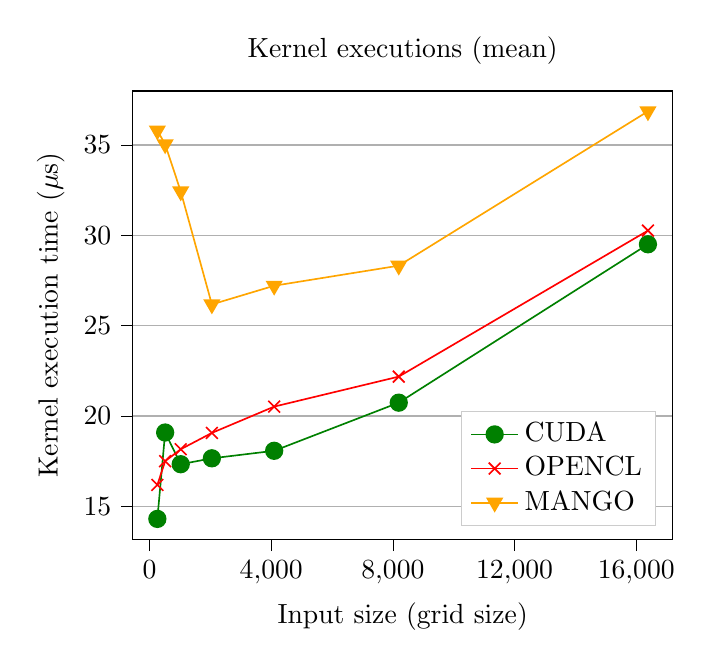
\begin{tikzpicture}

\definecolor{color0}{rgb}{1,0.647058823529412,0}

\begin{axis}[
legend cell align={left},
legend style={
  fill opacity=1,
  draw opacity=1,
  text opacity=1,
  at={(0.97,0.03)},
  anchor=south east,
  draw=white!80!black
},
tick align=outside,
tick pos=left,
title={Kernel executions (mean)},
x grid style={white!69.0196078431373!black},
xlabel={Input size (grid size)},
xmin=-550.4, xmax=17190.4,
xtick style={color=black},
y grid style={white!69.0196078431373!black},
ylabel={Kernel execution time ($\mu$s)},
ymajorgrids,
ymin=13.1755189830914, ymax=37.9917063550803,
ytick style={color=black},
scaled x ticks = false,
xtick={0, 4000, 8000, 12000, 16000},
]
\addplot [semithick, green!50.1960784313725!black, mark=*, mark size=3, mark options={solid}]
table {%
256 14.3035275
512 19.0845953667954
1024 17.3306496732026
2048 17.656685966634
4096 18.0730500490677
8192 20.7366837857667
16384 29.5047277512547
};
\addlegendentry{CUDA}
\addplot [semithick, red, mark=x, mark size=3, mark options={solid}]
table {%
256 16.1839365700861
512 17.4985770416025
1024 18.1579511051574
2048 19.0632247081712
4096 20.5183282178218
8192 22.1790555555556
16384 30.2621266070773
};
\addlegendentry{OPENCL}
\addplot [semithick, color0, mark=triangle*, mark size=3, mark options={solid,rotate=180}]
table {%
256 35.8026210691824
512 35.0376165354331
1024 32.4320626649077
2048 26.175443620178
4096 27.2096125186289
8192 28.3202890760466
16384 36.8636978381717
};
\addlegendentry{MANGO}
\end{axis}

\end{tikzpicture}
